\section{System design and composition}
\subsection{Model}
The system is modelled in two parts: the moving base and the\ldots
% TODO: describe the moving base, and the attachment, whatever it ends up being.
% Include physical models.


% Describe the states of the system.
We argue for the folloing five states of the system:
\begin{inline-enum}
\item waiting for a command;
\item moving to a destination;
\item following a navigation-line;
\item picking an object up; and
\item dropping an object off.
\end{inline-enum}
The relation between these five states are visually described in the state machine of Fig~\ref{fig:state_machine}.
\begin{figure*}[ht]
  \centering
  \begin{tikzpicture}
    \node[state, initial, accepting] (wait) {waiting for \\ command};
    \node[state, right of=wait] (move) {moving to \\ destination};
    \node[state, below of=move] (follow) {following \\ line};
    \node[state, right of=follow] (pickup) {picking \\ up object};
    \node[state, left of=follow] (dropoff) {dropping \\ off object};

    \path[->] (wait) edge node{Arrowhead \\ signal} (move)
    (move) edge[sloped] node{line detected \\} (follow)
    (follow) edge[sloped] node{station detection \\ (system w/o object)} (pickup)
    (follow) edge[sloped] node{station detection \\ (system w/ object)} (dropoff)
    (pickup) edge[sloped] node{object picked up \\} (move)
    (dropoff) edge[sloped] node{object dropped \\} (wait)
    ;
  \end{tikzpicture}
  \caption{High-level state machine of the system.}
  \label{fig:state_machine}
\end{figure*}
\subsubsection{Mobile platform}
The model used in this case is the unicycle model, due to the differential steering. 
This is because of the mobile platform has only two wheels/trucks and it is not able to apply any steering angle to its wheels. 
The only way this robot can change orientation is by giving different velocity on each wheel-driving servo on left- and right- side. 
With this feature it is also possible to change the orientation of the mobile platform without changing the position of the platform. 
I.e. the robot is able to spin while the right-hand sidewheels have the same velocity as the left-hand side wheels, in opposite direction. 

\begin{figure}[h!]
\centering
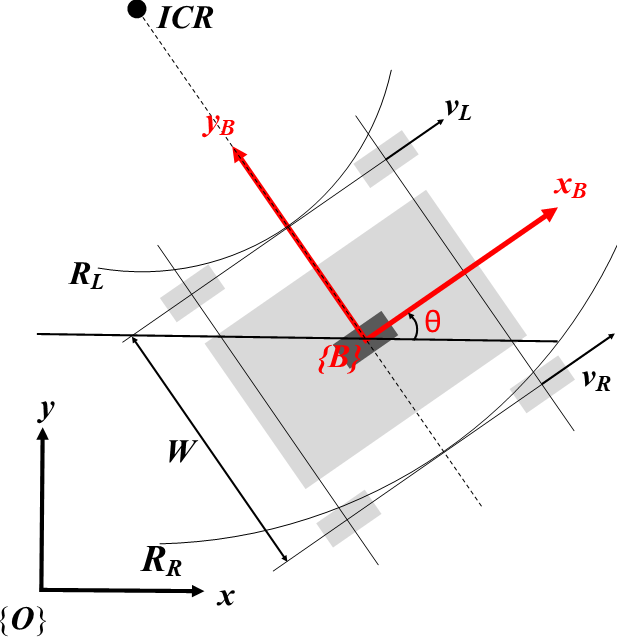
\includegraphics[width=0.4\textwidth]{sections/assets/car-unicycle.png}
\caption{Unicycle model of a car-like robot. 
$v_L$ and $v_R$ represent the left- and right-hand side wheels' velocities respectively. 
The robot follows a path around the instantaneous center of rotation (ICR) where $R_L$ and $R_R$ are the distances from left and right wheels to ICR respectively and $w$ is the distance between them.}
\label{fig:UnicycleModel}
\end{figure} 

As shown in Fig.~\ref{fig:UnicycleModel} The robot follows a curved path with the instantaneous center of rotation at its center. 
The left-hand side wheels have velocity $v_L$ and moves along an arc with radius $R_L$ during the time that right-hand side wheels moves along another arc with radius $R_R$ at the speed of $v_R$. 
The turning rate of the body is
        \begin{equation*}
            \dot{\theta}= \frac{v_L}{R_L} = \frac{v_R}{R_R}
        \end{equation*}
        since $R_R = R_L + W$ the expression can be simplified as
        \begin{equation}
            \dot{\theta}= \frac{v_R - v_L}{W} = \frac{v_\Delta}{W}\label{eq:ThetaDot3}
        \end{equation}
        the equations of motion for this model are
        \begin{eqnarray}
            \begin{aligned}
                \dot{x} &= v\,cos(\theta)\\
                \dot{y} &= v\,sin(\theta)\\
                \dot{\theta} &= \frac{v_\Delta}{W}
            \end{aligned}
            \label{eq:MotionEq3}
        \end{eqnarray}
        where the average velocity\parencite{Corke2011} is given by
        \begin{equation}
            v = \frac{v_R + v_L}{2} 
            \label{eq:av_velocity}
        \end{equation}{} 


\subsection{Simulation}
% Simulte the models from the previous section and show that it will work.
% Motivate regulation approach.

\subsection{Hardware}
% Explain the raspberry pi and it's attachments.

% TODO: remove this section; talk about software in `implementation.nix` instead.
\subsection{Software}

% TODO: rewrite/move elsewhere?
\subsubsection{System-external services}
The software environment generated for the Raspberry Pi automatically connects to Eduroam if credentials are available.
Eduroam places some limitations on connected clients: firewall, e.g.
To enable easy remote access to the system, a reverse SSH proxy is established with a known bastion host which has a static IP address.
By exposing this proxy via a known port on the bastion, any system connected to the Internet may trivially access the Raspberry Pi remotely via a static endpoint.
While not a necessity for the project itself, this external service is a great convenience for ad-hoc experiments and general system debugging.

% Explain the content of contrib/bastion.nix
